
\documentclass[letterpaper,twocolumn,10pt]{article}
\usepackage{usenix-2020-09}

% to be able to draw some self-contained figs
\usepackage{tikz}
\usepackage{amsmath}

% inlined bib file
\usepackage{filecontents}

% to include png figures
\usepackage{graphicx}

% Include the listings package and define code style
\usepackage{listings}
\lstdefinestyle{mystyle}{
    language=Python,
    basicstyle=\ttfamily,
    keywordstyle=\color{blue},
    commentstyle=\color{green},
    stringstyle=\color{red},
    breaklines=true,
    showstringspaces=false,
    numbers=left,
    numberstyle=\tiny,
    frame=single
}

%-------------------------------------------------------------------------------
\begin{document}
%-------------------------------------------------------------------------------

%don't want date printed
\date{}

% make title bold and 14 pt font (Latex default is non-bold, 16 pt)
\title{\Large \bf CYBR410 Group Project: Big Deployment}

%for single author (just remove % characters)
\author{
  {\rm Paul Aguilar}\\
  Front-End
  \and
  {\rm Nicholas Burlakov}\\
  Front-End
  \and
  {\rm Nehemiah Fiedls}\\
  Logging
  \and
  {\rm Eric Leachman}\\
  Orchestration
  \and
  {\rm Thomas Longwell}\\
  Defense
  \and
  {\rm Robert Rutherford}\\
  Defense
  \and
  {\rm Spencer West}\\
  Services
}

\maketitle

%-------------------------------------------------------------------------------
\begin{abstract}
%-------------------------------------------------------------------------------
The goal of this project is to work as a group with each member implementing a different aspect making up a larger deployment. 
\end{abstract}


%-------------------------------------------------------------------------------
\section{Introduction}
%-------------------------------------------------------------------------------
This project is designed to have groupmates work together to design and implement a full deployment. Each team mate was assigned a specific piece of the deployment as their responsibility and each section of this paper relates to a section of the deployment. Front-End is in charge of creating the user interface of the deployment as well as the web server that will host the services. The Services team then implemented an URL to physical location feature as well as a URL to current weather forecast converter. Behind the scenes the Defense team integrated an IP blocking honeypot to deter attacks, while Logging used a Sysdig script to keep a record of all traffic. This was handed to Orchestration, who spun up the servers on the designated IP assigned by the professor. 


%-------------------------------------------------------------------------------
\section{Orchestration}
%-------------------------------------------------------------------------------
The orchestration for this deployment concerns itself with two key areas. The first area, services, 
have been designed utilizing docker containers and docker compose for simple build up and tear down. 
Our docker compose solution utilizes two docker images, one running NGINX as a reverse proxy, 
and the other running a flask server locally which serves as an endpoint for the NGINX server. 

The second area, defense, utilizes OpenCanary and IPTables. While OpenCanary is also a docker container, the 
complexity in building it warrants its own separate orchestration. To accomplish this, we utilize 
some basic bash scripting to automate the necessary commands to run OpenCanary with the configuration and 
services required. We also include IPTables commands part of this bash script. These rules filter ports and 
drop traffic that attempts to enumerate OpenCanary and its ports. 

By automating most of the more complex tasks, our services and defenses can be deployed quickly 
and by a greater number of individuals, even those not intimately familiar with its inner workings. 
The use of docker containers and docker compose also allow our deployment to be mobile, only requiring 
prospective users to install a small number of programs (i.e., docker, docker compose, git). 




%-------------------------------------------------------------------------------
\section{Front end}

	The front end is designed around a few simple HTML template pages, stylized with a CSS style guide. There are three main templates and a variation on two – the first template is the index, a home page that is repeatedly linked on some blank links in the navigation bar. There are also two pages dedicated to the address and weather API’s. These pages have two versions, a search and an output template. The search template uses a simple form for the user to input a URL. The output template displays the results from the API call. These files are hosted via a flask server. \cite{grinberg2018flask}

	The flask server uses the render\_template and request objects to function seamlessly with the HTML and CSS. Following traditional directory organizations, a templates and static directory are used to hold those files for flask to access.
	\begin{verbatim}
	/app
    		- fServer.py
    	/templates
        - index.html
    	/static
		logo png’s
		/fonts
      	/styles
            	- style.css
	\end{verbatim}
Flask’s render\_template is used to display the correct HTML template in any given scenario, either from the hostWeather method or directly in the HTML links. The request object is used to handle the form submissions so that the user provided URL’s can be used by the API methods to generate the correct output. Both hostAddress and hostWeather use a similar method to pass the URL correctly depending on whether a POST request was made from a form submission, via requests request.form method or directly from the URL query string. From there the API methods are used to gather the data, which is the outputted using the render\_template method and displayed with in the output template.

% Include Python code snippet
\begin{lstlisting}[style=mystyle, caption=hostWeather method handles GET/POST requests, label=lst:python]

@app.route("/weather", methods=['GET', 'POST'])
def hostWeather():
    if request.method == 'POST':
        # Logic to handle form submission via POST request
        incomingHost = request.form['url']
    else:
        # Logic to handle GET request
        incomingHost = request.args.get('url', '')

    ipAddress = getIP(incomingHost)

    if checkCache(cacheW, incomingHost):
        weather = cacheW[incomingHost]
    else:
    	weather=getWeather(incomingHost)
    	addCache(cacheW, incomingHost, weather)

\end{lstlisting}

	While the host methods route to the correct output page, the remaining routes direct a user to the index or the search pages. The following sequence diagram shows the basic user interaction with the site:
\begin{figure}[htbp]
    \centering
    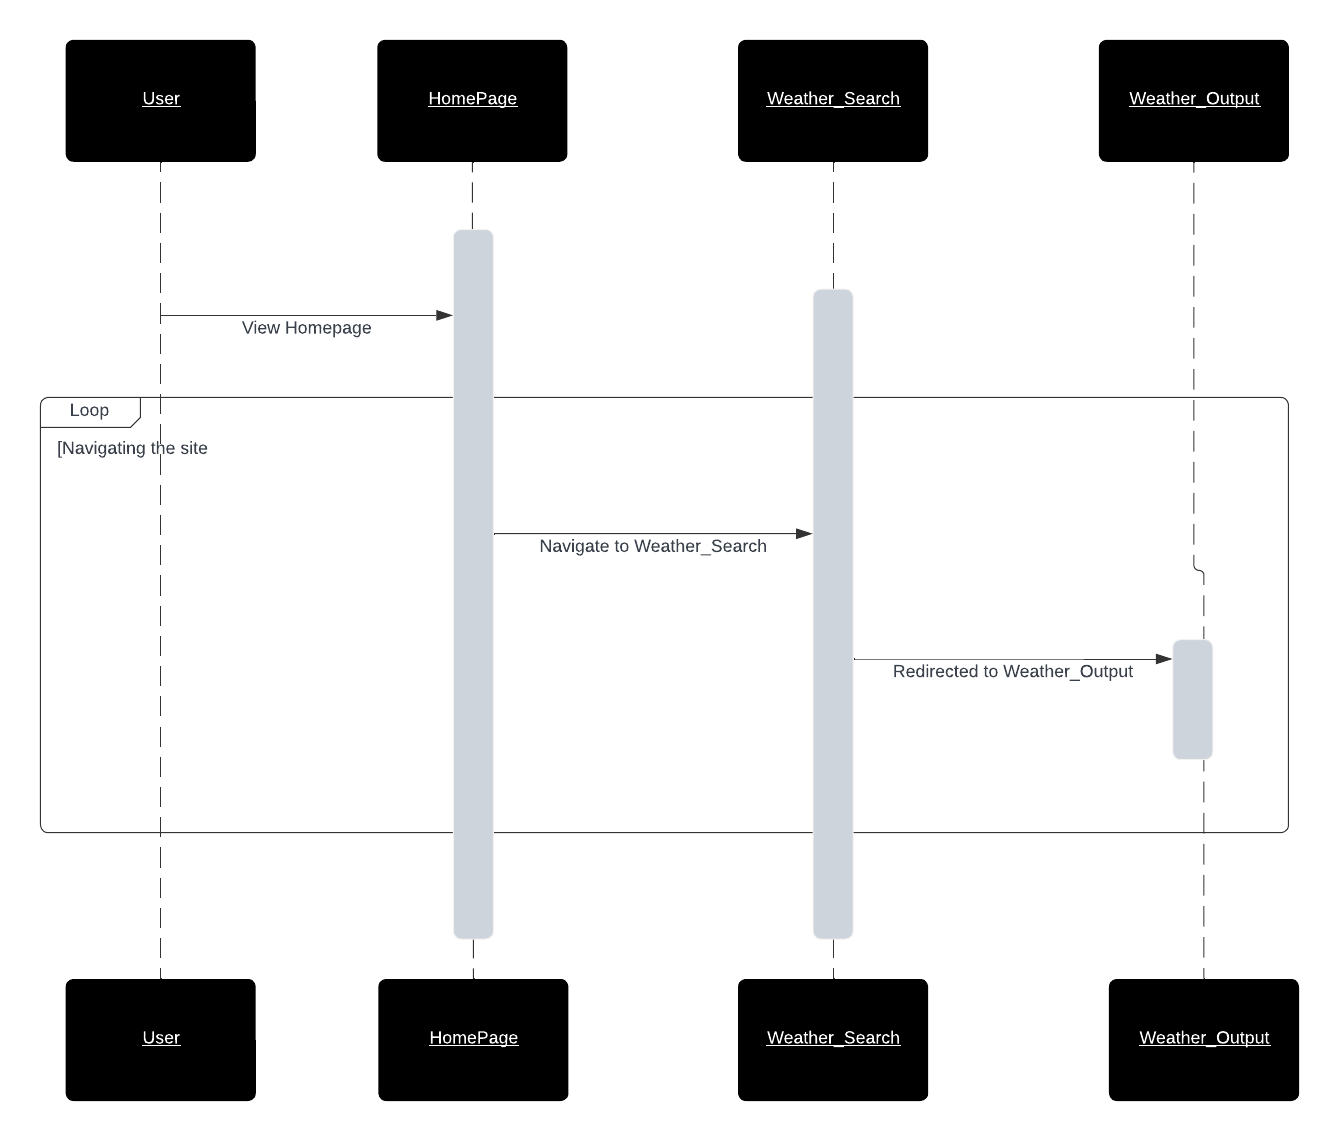
\includegraphics[width=0.5\textwidth]{sequenceD.png}
    \caption{Environment Diagram}
    \label{fig:example}
\end{figure}

%-------------------------------------------------------------------------------
\subsection{Evaluation Methodology \& Results}
%-------------------------------------------------------------------------------
\input{evalFrontend}
	

%-------------------------------------------------------------------------------
\section{Services}

	This web application incorporates two API's in a flask server. One service takes a URL and outputs the address of the registered owner based on the whois \cite{rfc3912} registry. The other uses that address and another weather API \cite{weather2009national,} to output the weather of that given location. It also uses a list to cache the data of visited sites, to improve performance. To do all this, the API is broken up in to multiple methods, which ultimately called by the hostWeather and hostAddress methods when a form submission is made on the webpage.
	
	The first method that is used is \verb+getIP()+, which first strips the incoming URL of any whitespace and then uses the socket library's \verb+gethostbyname()+ method to save the IP. This method is then used by both \verb+getWeather()+ and \verb+getAddress()+ in order to find the related information. \verb+getAddress()+ uses the subprocess' \verb+getstatusoutput()+ method to run the \verb+whois+ commandline tool to search for the registrar information based on the provided IP. It then splits the incoming tuple by a newline and parses out the different address fields, combines them and returns a whole address. 
	
	The getWeather method then passes that address in to a geocoding API to find the latitude and longitude of the address, which is required by the weather API that is used. The geocoding call returns a json file, that needs to be parsed and split between x and y coordinates correctly. The request's get method is then used to make an API call to weather.gov \cite{weather2009national} via the command line again. This outputs another json file that is then parsed to find the correct URL that contains the weather information. The get method is used once again on that forecast URL, which outputs the final json file, this is correctly parsed and returned as the weather for the given IP.

	The remaining methods handle the caching, either directly adding to it based on the correct list or traversing it to search for the given key which returns true or false. The host methods use this to first check the cache and then output the value based on the given key or add the key/value pair to the given cache if it isn't found. To summarize, this script creates a Flask web server that provides endpoints for IP address lookup and weather information retrieval, caching the results to improve performance. It also demonstrates how to integrate external APIs and system commands into a Flask application.


%-------------------------------------------------------------------------------
\section{Logging}

This is the logging section (miah)

%-------------------------------------------------------------------------------
\section{Defense}

In this section we will discuss the implementation of defense for our group project in detail. Our group's approach to defense includes a two part system, consisting of a honeypot and iptable rules to control traffic. The goal of the honeypot is to provide an avenue for investigation that distracts from the actual critical infrastructure. Once this unauthorized traffic occurs, the rules that we created drops the connection. This slows down or may entirely stop unauthorized users who have the intent to scan the server and try to connect or exploit it. With fake services on the honey pot, their attention will be diverted to multiple red herrings. This defensive approach assumes authorized users will know what is in scope and not try to connect to or scan the honeypot.

The honeypot we chose for this project is opencanary. Opencanary was selected because of our  familiarity with it, as well as its simplicity and interoperability with the rest of the group's implementation. It slots in easily because it’s built with docker, and allows our group to seamlessly integrate it with our other dockerfiles. This allows for quick configuration, and once the configuration file is set, building and running the dockerfile is easy. The ease of deployment works perfectly for the attacks that we anticipate later in the project, and will allow transferring of the honeypot to a new server to be easily handled with a single script. 

Traffic rules set by iptables include a very basic approach to discouraging traffic on the machine. Opencanary has enabled a large volume of ports that seem promising to exploit. After an initial scan, the attacker would recognize these and begin to press on these attack surfaces. Unbeknownst to them, all traffic going to these ports will be dropped with no reason or message given to the attacker. Using DROP instead of REJECT provides the client no insight into why their connection is unsuccessful. On their side, it just appears that their request is hanging forever. This simple yet effective measure is a major piece of our defensive strategy. Opencanary’s large volume of unnecessary ports in tandem with these rules will cause major disruptions to any penetration attempts, guaranteeing a strong level of security for the system. 



%-------------------------------------------------------------------------------
\bibliographystyle{plain}
\bibliography{refs}

%%%%%%%%%%%%%%%%%%%%%%%%%%%%%%%%%%%%%%%%%%%%%%%%%%%%%%%%%%%%%%%%%%%%%%%%%%%%%%%%
\end{document}
%%%%%%%%%%%%%%%%%%%%%%%%%%%%%%%%%%%%%%%%%%%%%%%%%%%%%%%%%%%%%%%%%%%%%%%%%%%%%%%%

%%  LocalWords:  endnotes includegraphics fread ptr nobj noindent
%%  LocalWords:  pdflatex acks
